% 三阶行列式的对角线法则
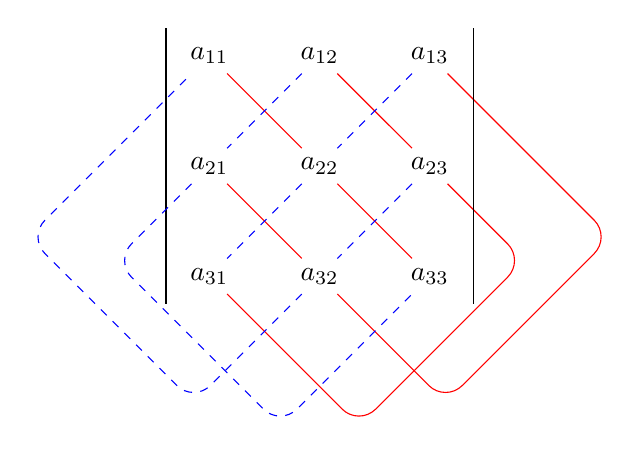
\begin{tikzpicture}

  \draw (-1.95,1.75) -- (-1.95,-1.75);

  \node at (-1.4,1.4) (a11) {$a_{11}$};
  \node at (0,1.4) (a12) {$a_{12}$};
  \node at (1.4,1.4) (a13) {$a_{13}$};

  \node at (-1.4,0) (a21) {$a_{21}$};
  \node at (0,0) (a22) {$a_{22}$};
  \node at (1.4,0) (a23) {$a_{23}$};

  \node at (-1.4,-1.4) (a31) {$a_{31}$};
  \node at (0,-1.4) (a32) {$a_{32}$};
  \node at (1.4,-1.4) (a33) {$a_{33}$};

  \draw[red] (a11) -- (a22) -- (a33);
  \draw[red,rounded corners=3mm] (a12) -- (a23) -- (2.6,-1.2) -- (0.5,-3.3) -- (a31);
  \draw[red,rounded corners=3mm] (a21) -- (a32) -- (1.6,-3) -- (3.7,-0.9) -- (a13);

  \draw[dashed,blue] (a13) -- (a22) -- (a31);
  \draw[dashed,blue,rounded corners=3mm] (a12) -- (a21) -- (-2.6,-1.2) -- (-0.5,-3.3) -- (a33);
  \draw[dashed,blue,rounded corners=3mm] (a23) -- (a32) -- (-1.6,-3) -- (-3.7,-0.9) -- (a11);

  \draw (1.95,1.75) -- (1.95,-1.75);
\end{tikzpicture}
